\documentclass[7x9]{times}

% use mit book class




\title{Penetration Testing and Ethical Hacking}
\author{Many authors}
%\institude{Nanjing University, China}
\date{\today}
\edition{2019 Edition}



%% For multiple indices:
%\usepackage{multind}
%\makeindex{topics}
%\makeindex{authors}

\def\taupav{\tau_{\mathrm{Pav}}}

\newbox\oiintbox
\setbox\oiintbox=\hbox{$\lower2pt\hbox{\huge$\displaystyle\circ$}
	\hskip-13pt\displaystyle\int\hskip-7pt\int_{S}\ $}
\def\oiint{\copy\oiintbox}

\def\boldnabla{\hbox{\boldmath$\displaystyle\nabla$}}

\nocropmarks

\usepackage{multind}
\makeindex{topics}
\makeindex{authors}

\usepackage{listings}
\lstloadlanguages{bash,Python}

\begin{document}

%[frontmatter] turns off chapter numbering and uses roman numerals for page numbers;
%[mainmatter] turns on chapter numbering, resets page numbering and uses arabic numerals for page numbers;
%[appendix] resets chapter numbering, uses letters for chapter numbers and doesn't fiddle with page numbering;
%[backmatter] turns off chapter numbering and doesn't fiddle with page numbering.

\titlepage

\begin{copyrightpage}
	\copyright\ 2019 Center for Cybersecurity and Cybersecurity Malaysia
	
	All rights reserved. No part of this book may be reproduced in
	any form or by any electronic or mechanical means (including
	photocopying, recording, or information storage and retrieval) without
	permission in writing from the publisher.
	
	
	This book was set in Syntax and Times Roman by the author.
	
	Printed and bound in the United States of America.
	
	Library of Congress Cataloging-in-Publication Data
	
	?? Book Title / ?? Book Author .\\
	\hspace*{6pt} p. cm.
	
	Includes bibliographical references and index.\\
	ISBN ???? 
	\vfill
	
	10\ 9\ 8\ 7\ 6\ 5\ 4\ 3\ 2\ 1\
	
\end{copyrightpage}

\tableofcontents
\listoffigures
\listoftables

\begin{contributors}[twocolumn]
	
	\contrib 
	Professor Alan Guth\\
	Center for Theoretical Physics\\
	Massachusetts Institute of Technology\\
	Cambridge, Massachusetts, USA
	
	\contrib 
	Professor Andrei Linde\\
	Department of Physics\\
	Stanford University\\
	Stanford, CA, USA
\end{contributors}


\begin{preface}
ALhamduiLlah. This book is based on lecture notes for \textit{TX6244:Ethical Hacking and Penetration Testing}, a course offered by Center for Cybersecurity(UKM) since 2014. This course is jointly developed by Center for Cybersecurity(UKM) and Cybersecurity Malaysia(CSM).

We hope this book will provide a good overview for students into the field of penetration testing and ethical hacking. We also hope these materials will encourage students to further explore this exciting field.

We try hard to be current up to 2019. However, this is a tall order with the amount of information available on the Internet. Al always, please inform of any errors or omissions to \url{zamri@ukm.edu.my}.

The book source code is available on \url{github.com/mohdzamrimurah/bukusiber}, and we welcome collaboration from all users.



\end{preface}


\chapter{Tools and Software}


\paragraph{Tools and Software} This chapter contain
information about basic essential tools and software for
penetration testing. Familiarity of these tools would make
it easier to conduct penetration testing.


\section{Linux}

Linux\cite{sobell2015practical,barrett2016linux} is an
operating system for computer, much like Window 10 or Mac
OSX. It is based on Unix. Linux was first developed in 1991
by Linus Torvalds, a Finnish graduate student. Currently it
is being develops and maintains by a group of software
developers head by Linus Torvalds. It is widely uses in
large technology companies like Google, Facebook, and
Amazon. Linux is widely use as enterprise servers for
enterprises daily operation. It is estimated that 70\% of
web servers use Linux, with 30\% using Window-based servers.

Linux is open source and free for everybody to use and to
modify. The open source creative license make it possible
for any person or organization to modify Linux to fit their
needs. For instance, Chinese government produce their own
modified version of Linux for the Chinese
market()\url{http://www.kylinos.com.cn/}). Similarly, many
organization such as NSA, Google(\url{gLinux}), Amazon have
customized Linux for their need.

There are many Linux distributions such as Ubuntu, SuSE,
Debian and Red Hat. Red Hat(Linux) is widely use as
enterprise servers, Ubuntu is widely by customer desktop and
Debian is normally uses by software developers. A Linux
distribution is a Linux operating system with other useful
software such such text editor, pdf viewer, browser, music
player and image processing. A Linux distribution is similar
to a PC with Window 10, Microsoft Office software and other
familiar software applications.

\index{topics}{Linux}
\index{topics}{Kali Linux}


\paragraph{Kali Linux}is a Linux distribution for
penetration testers. It consists of many widely used tools
for pentest. This distribution make it easy to use common
tools in a pentest. There are about 200+ tools in Kali Linux
for various stages of a pentest.

\section{git}

\paragraph{git}\cite{loeliger2012} is a source code
management tool. \url{github.com} is a git repository, where
software developers share their software source codes in the
Internet. \url{Github.com} host many open source pen test
tools projects such as \url{metasploit} and \url{nmap}. A
pen tester can clone the repository and install the software
on his machine. With this approach, the pen tester can
always use the latest version of the software.

A pen tester need to clone the repository from
\url{github.com}. An example for such action is given below
for cloning \url{nmap} repository.


\verb|git clone https://github.com/nmap/nmap.git|

% https://www.online-convert.com/
% take screen shot in png, convert to eps

\begin{center}
	\begin{figure}[ht]
		\includegraphics[width=\textwidth]{00.46.46_46.eps}
		\caption{github.com}
	\end{figure}
\end{center}


\index{topics}{git}
\index{authors}{Loeliger, Jon}

\section{Python}

\paragraph{Python} is a programming language, widely used in data science, deep learning and web development and software development. Recently, it has been used to develop tools for pen tests. Python is a scripting language, and easy to learn.



\section{Raspberry Pi}

\section{Cybersecurity News}

\section{Definitions}

\section{Web resources}


\section{Web Sites}

\section{Summary}

\begin{center}
	\begin{figure}[h]
		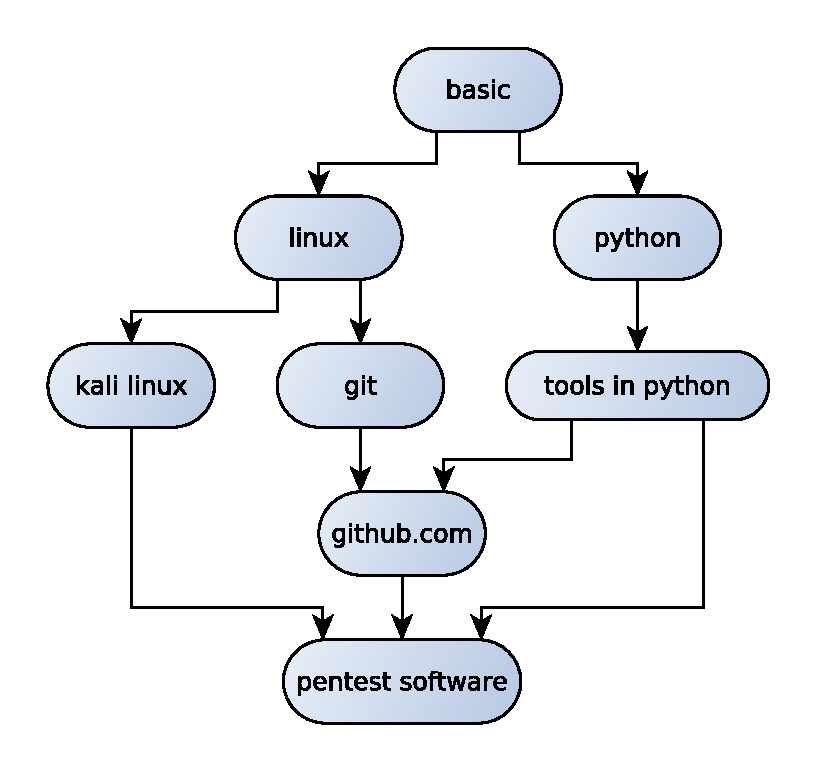
\includegraphics[width=\textwidth]{tools.eps}
		\caption{Basic tools for pen testers.}
	\end{figure}
\end{center}




\chapternotes

\chapter{Network Basic}

\section{Network}
\section{How Internet works}
\section{IP, DNS}
\section{Web servers}


\chapter{Network}

\section{Reconnaissance}
\section{Scanning}
\section{Enumeration}
\section{Vulnerability Assessment}



\chapter{Web Apps}
\section{Web Apps}
\section{Reconnaissance}
\section{Scanning}
\section{Enumeration}
\section{Vulnerability Assessment}

\chapter{Wireless}



\chapter{Mobile}

\chapter{Server and Desktop}

%\nocite{*}
%\bibliographystyle{mit-chicago}
\bibliographystyle{unsrt}
\bibliography{buku}


\printindex{authors}{Author Index}
\printindex{topics}{Topic Index}

\end{document}
